\documentclass[9pt,twocolumn,twoside]{../../styles/osajnl}
\usepackage{fancyvrb}
\journal{i524} 

\title{ On-line advertisement click prediction }

\author[1,*]{Sahiti Korrapati}

\affil[1]{School of Informatics and Computing, Bloomington, IN 47408, U.S.A.}

\affil[*]{Corresponding authors: sakorrap@iu.edu, S17-IR-2013}

\dates{S17-IR-2013, May 04, 2017}

\ociscodes{Hadoop, On-line Advertisement, BigData, Cloudmesh Client, Ansible, Chameleon Cloud, Apache Pig, HDFS, MapReduce, I524}

% replace this with your url in github/gitlab
\doi{Report: \url{https://github.com/cloudmesh/sp17-i524/tree/master/project/S17-IR-2013/report/report.pdf}
\newline Code: \url{https://github.com/cloudmesh/sp17-i524/tree/master/project/S17-IR-2013/code}}

\begin{abstract}
This project aims at predicting the most suitable advertisements from an available pool with unique ad\_id to be displayed on a web-page. Each webpage has a window to display six advertisements and each window has a display\_id and each advertisement is associated to. So, top six advertisements are selected based on highest relevance with the web page. Relevance factor is calculated by ranking ads based on the likelihood of click if displayed. Data is obtained as CSV files from Kaggle Data sets and is stored in Hadoop Data File system(HDFS). In this project, Ansible along with Cloudmesh client and Bash shell is used to automate the deployment of cloud architecture and necessary software on Chameleon cloud and for performance bench-marking. Apache Pig on Hadoop was chosen for data exploration and analysis. Pig engine executes the data flows in parallel by making use of Hadoop MapReduce framework.
\newline
\end{abstract}
\setboolean{displaycopyright}{true}

\begin{document}
\maketitle
\section{Introduction}
It has been analyzed that an average American spends about 23 hours per week surfing on-line \cite{news-social-media}. This on-line user activity is being captured by companies to perform analyzes for advertisement, recommendation and many other purposes. This has given rise to the field of "Web Analytics" and one such application is Ad Click prediction.

Many measures are available to assess the ad performance. One popular measure to assess the immediate ad response is click-through rate (CTR) of the advertisement \cite{dictionary-clickThrough} which is defined as the ratio of the number of clicks on an ad to the number of times the ad is shown, expressed as a percentage. In this project, I attempted to make use of CTR along with ranking each ad based on the level of relevance to the original web page. For calculating the CTR, historical data of user activity needed to be explored \cite{wiki-clickThrough}.

The user activity data from web that is available for prediction is enormous. Every page view and advertisement click is tracked by web browsers. This data for millions of users potentially generates enormous volumes. The current project uses big-data stack i.e Apache Pig along with Hadoop to analyze predict. Hadoop is a large scale data processing system which runs on parallel processing to handle huge volumes of data. Pig is a high level language which runs on top of Hadoop's HDFS infrastructure. Pig Latin scripts are simple to comprehend and SQL-like queries which can process large volumes of data.

Ansible along with Cloudmesh client is used to deploy the software on Chameleon Cloud. Ansible is a cloud automation tool which allows easy deployment and configuration of multiple servers in one step. Cloudmesh allows us to deploy and install Hadoop instances on a cluster with any number of nodes.

\section{Background}
\subsection{About Data}
The data set in this paper is taken from Kaggle data sets. It is released by Outbrain which has 2 Billion page views and 16,900,000 clicks of 700 Million unique users, across 560 sites \cite{kaggle-outbrain}.

The data set contains a sample of users’ page views and clicks, as observed on multiple publisher sites in the United States between 14-June-2016 and 28-June-2016. Each viewed page or clicked recommendation is further accompanied by some semantic attributes of those documents \cite{kaggle-outbrain}. It contains numerous sets of content recommendations served to a specific user in a specific context. Each context (i.e. a set of recommendations) is given a display\_id. In each such set, the user has clicked on at least one recommendation. Our task is to rank the recommendations in each group by the decreasing predicted likelihood of being clicked \cite{kaggle-outbrain}.

Each user in the dataset is represented by a unique id (uuid). A person can view a document (document\_id), which is simply a web page with content (e.g.  a news article). On each document, a set of ads (ad\_id) are displayed. Each ad belongs to a campaign (campaign\_id) run by an advertiser (advertiser\_id). Figure \ref{fig:OutbrainData} shows the fields in our dataset. Metadata about the document is also provided, such as which entities are mentioned, a taxonomy of categories, the topics mentioned, and the publisher \cite{kaggle-outbrain}.

\begin{figure}[hptb]
\centering
\includegraphics[width=\linewidth]{images/page_view.png}
\caption{Displaying Source, Publisher, Document, Promoted content set and items \cite{kaggle-outbrain}}
\label{fig:OutbrainData}
\end{figure}

\subsection{Ansible and Cloudmesh client toolkit}
Ansible is an opensource cluster management tool which has the ability to maintain a fully immutable server architecture and design. It is a simple automation engine that automates cloud provisioning, configuration management, application deployment, intra-service orchestration \cite{www-ansible-work}. It doesn't use agents or custom security infrastructure, so it's easy to deploy by using "YAML-language" (YAML, in the form of Ansible Playbooks). 

Using Ansible, users can define any number of IP Addresses in hosts file, and create custom groups for specific tasks. These group names can be referred to in the YAML file to perform a specific set of tasks in each of the virtual machines. Ansible also has options to define specific roles for each task and make YAML files dynamic using global variables.

With Cloud mesh, the deployment becomes even simpler and easier. Cloud mesh client toolkit, a lightweight client interface to access heterogeneous clouds, clusters, and workstations, available as API, commandline client and commandline shell. Their quick start user manual has everything that is needed to start using the tool \cite{www-cm-docs}.

The current project uses Cloudmesh's "cm" command to perform multiple tasks including cluster deployment, installing and configuring Hadoop and Pig, enabling the cloud nodes to be able to ssh with each other and assigning floating IP addresses to each node. The configuration of the cluster can be defined in Cloudmesh's YAML file and accordingly the cluster will be created with the given OS and type.

\subsection{Hadoop in Big-data}
Hadoop is a distributed platform designed to help manage and analyze massive data-sets that are too big or costly to put in relational databases. Rather than storing and processing the whole data in one high-end computer, data can be spread across many smaller nodes. By spreading the data across multiple nodes, the storage as well computational speed can be scaled by parallel processing \cite{www-thinkbig}.

Hadoop framework is developed for distributed processing of large data sets across clusters of computers using simple programming models. It can scale up from single servers to thousands of machines, each offering local computation and storage. The library is designed to deliver a highly available service on top of a cluster of computers, each of which may be prone to failures \cite{www-readwrite}.

\subsection{HDFS and MapReduce}
Hadoop Distributed File System (HDFS) and the MapReduce parallel processing framework are two primary components at the core of Apache Hadoop. Figure \ref{fig:HadoopArchitecture} shows the high level architecture of Hadoop in regards to HDFS and MapReduce 

\begin{figure}[hptb]
\centering
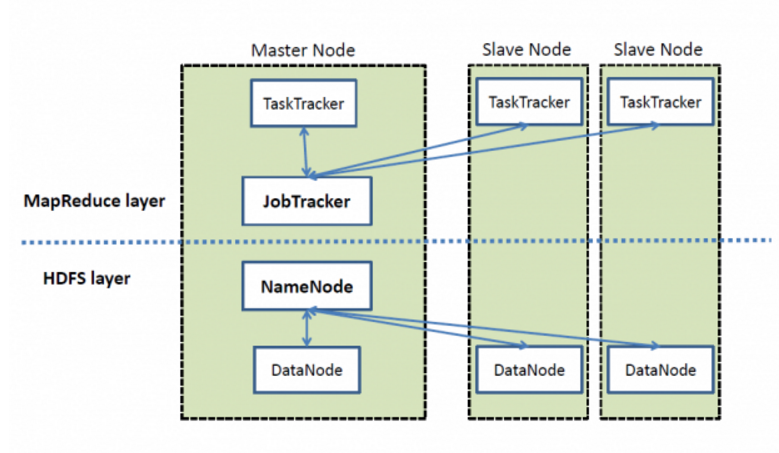
\includegraphics[width=\linewidth]{images/HadoopArch.PNG}
\caption{ High Level Architecture of Hadoop \cite{www-opensource}}
\label{fig:HadoopArchitecture}
\end{figure}

HDFS is a distributed, scalable, and portable file-system for Hadoop framework.
Files are broken into blocks and spread across nodes in the cluster in HDFS. The blocks are also replicated on different nodes so that even if one of the nodes fails another one of the live nodes still has a copy of the data. There is a NameNode and DataNodes. The NameNode maintains the references on the file split up in blocks across nodes in the cluster. While reading, client process contacts the NameNode for this metadata and ask the corresponding DataNodes for those blocks for reading \cite{www-thinkbig}.
MapReduce is for processing files stored in a distributed environment like HDFS. A typical MapReduce application has two functions, a Mapper and a Reducer. Mappers and Reducers run as tasks on nodes in the cluster. Two processes JobTracker and TaskTracker manages MapReduce framework. The JobTracker is the master process that coordinates the Map and Reduce tasks sent across the cluster.

\subsection{Apache Pig}
Pig platform is designed to work with large data sets for analysis. The Pig dialect is called Pig Latin, and the Pig Latin commands get compiled into MapReduce jobs that can be run on a suitable platform, like Hadoop. Figure \ref{fig:Pig} illustrates how it makes use of MapReduce framework.

\begin{figure}[hptb]
\centering
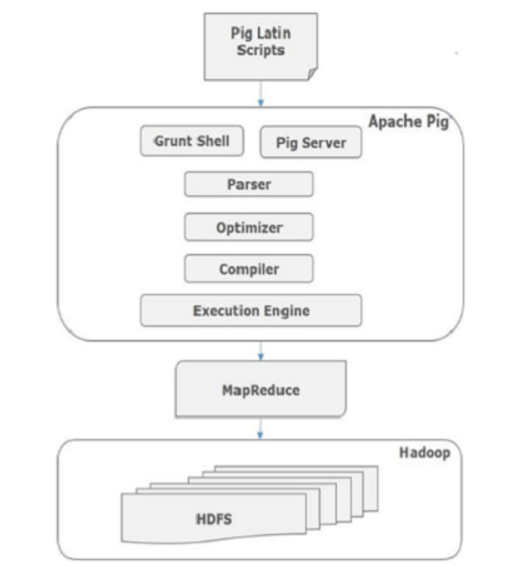
\includegraphics[width=\linewidth]{images/PigArch.PNG}
\caption{ Architecture of Apache Pig \cite{www-opensource}}
\label{fig:Pig}
\end{figure}

Pig is a high level language which is similar to SQL in syntax. The structure of Pig is designed such that the Pig scripts are made amenable for parallel processing. Pig scripts are automatically optimized so that the programmers can focus on semantics rather than efficiency \cite{www-pig-apache}. Pig also has options to create user defined functions to perform complex tasks using Pig.

\subsection{Chameleon cloud}
Chameleon Cloud is a cloud platform offered for research purposes free of charge. It is maintained by the Chameleon community and is funded exclusively for use by students and faculty by the National Science Foundation. Chameleon Cloud is deployed at University of Chicago and Texas Advanced Computing Center, and consists 650 multi-core cloud nodes, 5PB of total disk space, and leverage 100 Gbps connection between the sites. 

The current project uses a cluster created on Chameleon cloud instance with three virtual machines on which Hadoop operates. Ubuntu 14.04 was installed on these machines with 20 GB disk space and 2 GB ram each.

\subsection{Data Analysis}
Though page\_views data is available, it has been excluded from analysis since the data was in orders of 100s of gigabytes for just 2 weeks. With the resources available we could only process two days of data for analysis. The prediction will be low in confidence if only two days are considered. Since the objective was to produce a reliable prediction of Ad ids with given resources, it was chosen to predict the more likely ads by relevance factor. Data was analyzed using Apache Pig in the MapReduce mode. Clicks\_train and events files were joined to get a list of documents to make the predictions. The above list was joined to documents\_events, documents\_categories and documents\_topics to generate a master dataset of all the required documents, their topics, categories and entities. The data in promoted\_content was joined with the data in documents\_events, documents\_categories and documents\_topics to generate a dataset which has all advertisement ids and their related document entity, topic and category. A master join between the two lists on the event, topic and category ID was performed to get matching document IDs. On this data, relevancy score for each match was calculated by multiplying the confidence levels. The final list was grouped by document ID and top six matching ad\_ids were generated based on the highest relevance score. These ads are the recommendations for each page. This recommendation engine is purely based on matching the association probabilities provided for web pages and advertisements with different topics, events and categories.

\section{Setup and Configuration}
This project was setup using Ansible and Cloudmesh Client. Cloudmesh client was used to install and deploy Hadoop clusters on Chameleon Cloud. Ansible was then configured to perform a set of tasks on the namenode of the server. File movement was handled using Ansible playbooks. The final Pig script was run on the namenode Hadoop server using automated Ansible scripts.

Multiple configurations were used for bench-marking the clusters, from m1.medium to m1.xlarge clusters with 1 to 10 nodes on Chameleon Cloud. One of the nodes in each cluster was configured to act as namenode and the rest as datanodes. The details of each flavor are given in Table 1, 2 and 3. With medium and large clusters it took extremely long time to do the analyses. So, we set our default configuration to deploy clusters with extra large clusters.
\begin{table}
\begin{tabular}{|c|c|c|c|}
\hline
    Flavor & m1.medium & m1.large & m1.xlarge \\ \hline
    Server & Ubuntu14.04 & Ubuntu14.04 & Ubuntu14.04 \\ \hline
    VCPU & 2 & 4 & 8 \\\hline
    Ram & 4 GB & 8 GB & 16 GB \\\hline
    Disk & 40 GB & 80 GB & 160 GB \\\hline
\end{tabular}
\caption{Virtual Machine Configuration}
\end{table}
\subsection{Deployment}

\section{Work Flow}
The deployment of clusters was done using Cloudmesh client's "cm deploy" command. A three node Hadoop cluster is created and enabled cross SSH between the nodes so that they will be able to communicate with each other. Next step was to use Ansible to transfer the data files and Pig script to cloud. Once this data transfer was done, Ansible scripts were used to move the files from the cloud to HDFS. The pig script was run using Ansible from the local system and timed for bench-marking. The final step was to transfer the output files back from hdfs to local system using Ansible.

\section{Experiments and Results}
Multiple experiments were conducted using different sizes of input data on different clusters. Deployment and performance results were used to benchmark Cloudmesh client and Chameleon cloud. Then performance bench-marking was done for an incremental number of web pages. The results were produced based on the time taken to predict the most likely to be clicked Ad for different number of web pages. Each document ID corresponds to a page that needs predictions and a list of 6 Ad\_id are predicted for each document\_id based on relevance score calculated. The score was calculated using the confidence levels given for different relevance factors. The relevance factors included the topic, entity and category to which each web page and ad was probable to belong. The time taken to deploy the clusters and to move the data were also recorded for analysis.

\subsection{Deployment bench-marking}
Cluster was deployed on Chameleon cloud with Hadoop and Pig for conducting analyses. Deployment bench-marking was done on clusters with different flavors of chameleon cloud nodes including m1.large and m1.xlarge. Time taken for deploying Clusters with 1 to 10 nodes was noted to check the trend of increase. This trend is presented in Fig. \ref{fig:dep_time}. The time taken to deploy a Hadoop cluster can be skewed by multiple things including network connectivity and cluster latency. In general, we observed an increasing trend in the deployment time of the clusters as the number of nodes increased. 

\begin{figure}[hptb]
\centering
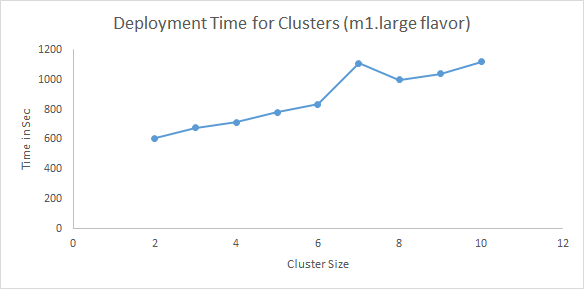
\includegraphics[width=\linewidth]{images/dep_time.png}
\caption{ Benchmarking Results: Time taken for Deploying Hadoop and Pig}
\label{fig:dep_time}
\end{figure}
\subsection{Moving files}
Two separate time readings were taken, to move data along with other binary files to namenode of the Hadoop cluster and then to move data to HDFS from namenode. This is performed on the cluster with m1.xlarge flavor. Data movement entirely depends upon network connectivity on both ends, and there were no notable trends observed in the time taken for moving to HDFS across different configurations with an average of 61 seconds. The time taken to move data to the cloud was irrespective of the cluster size as files needed to be put only on namenode. The average time taken for moving files to the namenode on chameleon cloud was 881 seconds. 

Figure Fig.\ref{fig:deployment_timetrend} compares the time taken for deployment, moving files to cloud and then moving the data files to HDFS.

\begin{figure}[hptb]
\centering
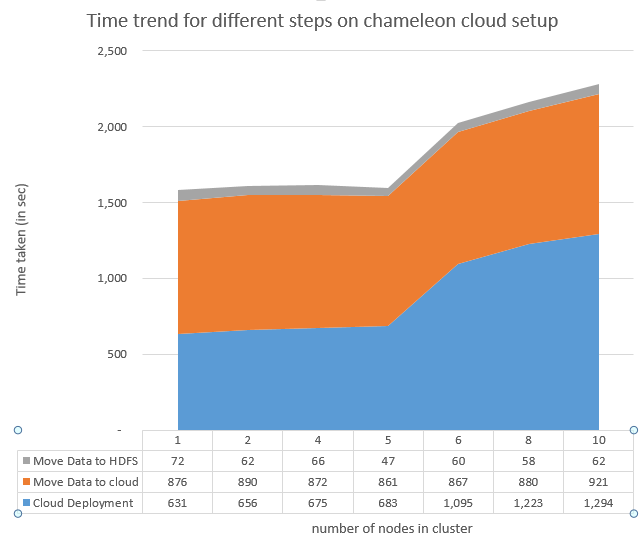
\includegraphics[width=\linewidth]{images/deployment_timetrend.PNG}
\caption{ Benchmarking Results: Time comparison for deploying clusters, moving file to cloud, moving data to HDFS}
\label{fig:deployment_timetrend}
\end{figure}

\subsection{Performance bench-marking}
Pig scripts were written to analyze the data that was moved to HDFS. The script takes input from HDFS location, performs a series of joins and filters out some data, and dumps the output to a HDFS location. Time taken for this entire process is recorded using time command of Linux shell. In order to automate this, the Pig script was looped in a bash script by giving the number of records to process as an input variable. 

Figure Fig.\ref{fig:xlarge_20k} compares time taken for predicting top six advertisements for different cluster sizes with m1.xlarge cluster flavor. From the figure, the performance results show that it scaled linearly up to 20000 web pages. The performance also depends various things such as network connectivity, and there was a notable decrease in time taken as the cluster size increases.The graphs are plotted for time versus the number of web pages to which predictions are made.

We can also observe that in figure Fig.\ref{fig:xlarge_20k} time taken for predicting using Pig with data files in and outside HDFS. In local, the data files are kept outside HDFS and output is written to a file outside HDFS. Whereas in 1 node, input files are put in HDFS and output is also stored to HDFS. This can be used to illustrate how the performance of Pig improves with HDFS.

\begin{figure}[hptb]
\centering
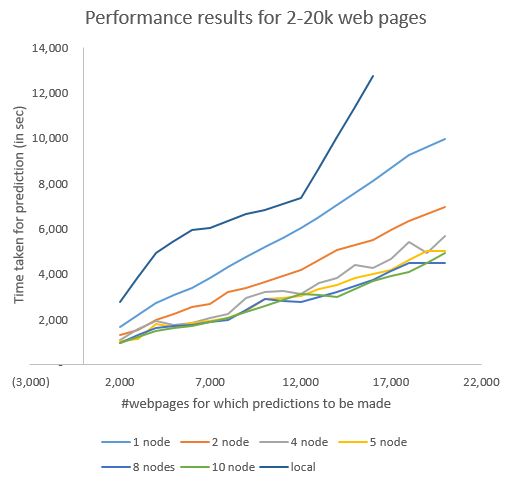
\includegraphics[width=\linewidth]{images/xlarge_20k.PNG}
\caption{ Benchmarking Results: Time taken for predicting best six Ads for each webpage}
\label{fig:xlarge_20k}
\end{figure}

A different plot is plotted to capture the time taken for different cluster sizes from 20,000 web pages on wards. Figure Fig.\ref{fig:xlarge_100k}

\begin{figure}[hptb]
\centering
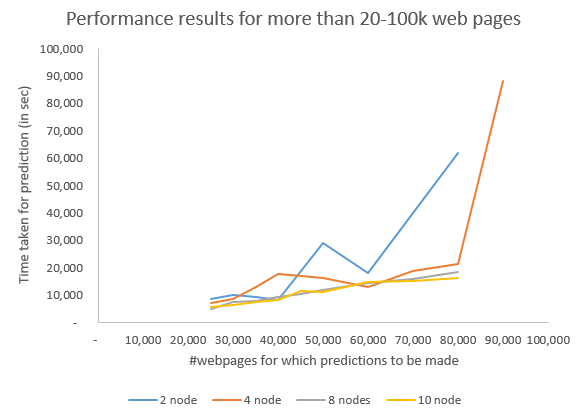
\includegraphics[width=\linewidth]{images/xlarge_100k.PNG}
\caption{ Benchmarking Results: Time taken for predicting best six Ads for each webpage}
\label{fig:xlarge_100k}
\end{figure}

\section{Conclusion}
Apache Hadoop technologies can be used to process large volumes of data in parallel to make quick analyses. Apache Pig is an add-on for Hadoop, which is a high level language for writing queries to process data. Apache Pig is efficient in query optimization and enables parallelism for its processing. It was even more efficient when data files were available in HDFS and output is written to HDFS as the time taken for either loading and/or storing significantly improved. The current project used Apache Hadoop and Pig to process large data related to online advertisement prediction. Online advertisement is one space where large amounts of data is collected and it demands the use of Hadoop like parallel processing and distributed systems to get meaningful insights from the data economically. 

As we can see from the results, Apache Pig was able to handle reasonably large sized files in short times. The processing time increased as the input query size increased. These nodes can be horizontally and vertically expanded to utilize the full extent of Hadoop's parallel processing capabilities in order to scale up. 

\section{Future work}

Planning to conduct predictions based on Ensemble methods. One way to predict is through click-through rate and one way is to predict by relevance factor. Using relevance factor as one of the attributes along with platform, user id and geo-location, logistic regression can be run to predict if the top ad ids generated by relevance factor to be included in the list or not. Since all that information is given in page\_views file which is in order of 100s of gigabytes for just 2 weeks data, we need larger clusters. 

\section*{Acknowledgements}
The author thanks Professor Gregor Von Laszewski and all the AIs of big data class for the guidance and technical support.

% Bibliography
\bibliography{references}
 
\section*{Author Biographies}
\begingroup
\setlength\intextsep{0pt}
\begin{minipage}[t][3.2cm][t]{1.0\columnwidth} % Adjust height [3.2cm] as required for separation of bio photos.
  \noindent
  {\bfseries Sahiti Korrapati} is pursuing her MSc in Data Science from
  Indiana University Bloomington
\end{minipage}
\endgroup
\newpage
\appendix
\section{Execution instructions}
This project requires Ubuntu 16.04 LTS (Xenial Xerus) machine. The file requirements.txt provided in Code repository can be used to install required modules in a virtual environment virtualenv. ReadMe file is provided in Code repository should be referred to deploy, analyse and benchmark.
\subsection{List available definitions} To list already defined clusters, stacks and sec groups
\newline cm cluster avail - for cluster definitions
\newline cm hadoop avail - for hadoop stack definitions
\newline cm secgroup list - for secure groups

\subsection{Cluster delete} To delete a cluster in use:
\newline cm cluster delete
\subsection{Change Cluster} To use a cluster other than the one in use.
\newline cm cluster use <cluster-xyz>
\subsection{List cluster nodes} To list current cluster nodes
\newline cm cluster nodes - generally first node is namenode and rest are datanodes
\subsection{List node details} To list the details of a node
\newline cm vm list |grep <nodename>
\subsection{ssh node} To ssh to any node
\newline cm vm ssh <nodename>
\subsection{Change to hadoop user} To change to hadoop user from cc user on chameleon cloud
\newline sudo su - hadoop
\subsection{Kill benchmark script} To kill benchmarkscript
\newline ps -ef|grep pig.sh
\newline kill -9 <process-id> 
\subsection{Time taken for each iteration} time taken to predict for 1000 webpages is 1000 iteration
\newline cat \/home\/hadoop\/nohup.out
\subsection{Output files} To see the output files
\newline hdfs dfs -cat /outbrain/<iteration-number> (in cluster node)
\section{Directory Structure}
The Code directory /project/S17-IR-2013/code contains several sub directories. 
\subsection{./} Contains all ReadMe, requirements.txt and copy\_repository\_files.sh
\newline copy\_repository\_files.sh copies all the files to outbrain directory in HOME directory. If outbrain directory already exists, then it takes the backup of the existing directory.
\subsection{./scripts/} Contains all shell and bash scripts. All the scripts are put in sub directories.
\subsection{./scripts/deploy/} Contains scripts for deploying cluster
\newline install\_hadoop\_pig.sh is hard coded to deploy m1.xlarge cluster on Chameleon clod and installs required software. Number of nodes should be provided as an argument and it is configured to time the deployment.
\newline re\_deploy\_cluster.sh deploys one more cluster along without disturbing the existing cluster. It also requires number of nodes as the argument and is configured to deploy m1.xlarge cluster on Chameleon cloud along with required software
\subsection{./scripts/benchmark/} Contains script for performance bench-marking
\newline benchmark\_pig.sh is a bash script for performance Bench-marking. It is hard coded to run in a loop for 1000 to 10000 web pages with a step size of 1000.
\subsection{./scripts/utils/} Miscellaneous scripts used for automation
\newline replace\_namenode.sh is for replace namenode details in pigscript and hosts file after deploying the cluster. 
\subsection{./conf/} Contains all configuration file templates
\newline hosts file is for configuring the ip address to which files needs to be moved
\subsection{./playbooks/} Contains all Ansible YAML files
\newline move\_data.yml is for moving files from local machine to namenode of the cluster in use. It takes input from hosts file
\newline move\_date\_hdfs.yml is for moving data to HDFS from namenode. It also takes input from hosts file.

\end{document}

